%ci sono delle pagine su composti ionici e molecolari da scrivere dopo
\subsection{Definizioni preliminari}
\textbf{DEF} Si dice \textbf{valenza} la capacità di un atomo di combinarsi con qualche altro atomo. In particolare essa esprime il numero di atomi di idrogeno con cui si può legare:
$$\ce{HCl} \rightarrow \text{un cloro legato a un idrogeno} \rightarrow \text{il cloro è monovalente}$$
$$\ce{H_2O} \rightarrow \text{un ossigeno legato a due idrogeni} \rightarrow \text{l'ossigeno è bivalente}$$
$$\ce{NH_3} \rightarrow \text{un azoto legato a tre idrogeni} \rightarrow \text{l'azoto è trivalente}$$
$$\ce{CH_4} \rightarrow \text{un carbonio legato a quattro idrogeni} \rightarrow \text{il carbonio è tetravalente}$$

\textbf{DEF} Si dice \textbf{stato} o \textbf{numero di ossidazione} la carica elettrica reale o formale di un atomo nei suoi composti ($+1,+2,+3$ o $-1,-2,-3$ ecc.)

\vspace{0.2cm}I numeri di ossidazione sono veri solo per i composti ionici, cioè questi possono effettivamente essere descritti in termini di cessione e acquisto di elettroni tra gli atomi che li compongono, ovvero all'interno di tali composti troviamo ioni. Nei composti molecolari invece sono solo una formalità, un artificio che usiamo per fare i bilanciamenti, dato che in essi avviene solo una parziale separazione di carica dovuta alla differenza di elettronegatività.

\vspace{0.2cm}Gli atomi neutri hanno numero di ossidazione 0, in quanto hanno stesso numero di elettroni e protoni. Pertanto valori positivi del numero di ossidazione indicano che l'atomo ha ceduto elettroni e quindi ha un eccesso di carica positiva, valori negativi che li ha ricevuti e quindi ha un eccesso di carica negativa.

Nei composti ionici il numero di ossidazione coincide con la carica degli ioni:

\begin{center}
  \begin{tabular}{|l|ll|ll|}
    \hline
    composto & numero (stato) & \hspace{-0.4cm} di ossidazione & numero (stato) & \hspace{-0.4cm} di ossidazione\\
    ionico & del catione & & dell'anione & \\
    \hline
    &&&&\\[-0.4cm]
    NaCl & \hspace{1cm}Na$^+$ & $\boldsymbol{+1}$ & \hspace{1cm}Cl$^-$ & $\boldsymbol{-1}$\\
    \hline
    &&&&\\[-0.4cm]
    CaCl$_2$ & \hspace{1cm}Ca$^{2+}$ & $\boldsymbol{+2}$ & \hspace{1cm}Cl$^-$ & $\boldsymbol{-1}$\\
    \hline
    &&&&\\[-0.4cm]
    AlCl$_3$ & \hspace{1cm}Al$^{3+}$ & $\boldsymbol{+3}$ & \hspace{1cm}Cl$^-$ & $\boldsymbol{-1}$\\
    \hline
  \end{tabular}
\end{center}

Nei composti molecolari il numero di ossidazione è assunto uguale in valore e segno alla carica che avrebbero gli atomi del composto se esso fosse considerato ionico.
In questo caso il numero di ossidazione rappresenta una carica elettrica
formale e non una realtà fisica:

\begin{center}
  \begin{tabular}{|l|ll|ll|}
    \hline
    composto & numero (stato) & \hspace{-0.4cm} di ossidazione & numero (stato) & \hspace{-0.4cm} di ossidazione\\
    molecolare & del catione & & dell'anione & \\
    \hline
    &&&&\\[-0.4cm]
    HCl & \hspace{1cm}H$^+$ & $\boldsymbol{+1}$ & \hspace{1cm}Cl$^-$ & $\boldsymbol{-1}$\\
    \hline
    &&&&\\[-0.4cm]
    H$_2$O & \hspace{1cm}H$^+$ & $\boldsymbol{+1}$ & \hspace{1cm}O$^{2-}$ & $\boldsymbol{-2}$\\
    \hline
    &&&&\\[-0.4cm]
    ClO$_3^-$ & \hspace{1cm}Cl$^{5+}$ & $\boldsymbol{+5}$ & \hspace{1cm}O$^{2-}$ & $\boldsymbol{-2}$\\
    \hline
  \end{tabular}
\end{center}

Una reazione redox  o di ossidoriduzione è una reazione in cui almeno due dei reagenti abbiano stato di ossidazione diverso da quello che hanno nei prodotti. In altre parole ci deve essere almeno una specie che cede elettroni e una che li riceve (tra poco diremo che, rispettivamente, almeno una si ossida e almeno una si riduce).

In queste reazioni avvengono scambi di elettroni, per cui se un elemento cede elettroni ce ne deve essere un altro che li acquista (non possono essere trasmessi nel mezzo circostante), cioè non esistono reazioni spontanee di sola ossidazione o di sola riduzione.

\vspace{0.2cm}\textbf{DEF} Si dice che una specie si \textbf{ossida} quando cede elettroni, dunque ossidarsi significa perdere elettroni.

\vspace{0.2cm}\textbf{DEF} Si dice che una specie si \textbf{riduce} quando acquista elettroni, dunque ridursi significa ricevere elettroni.

\vspace{0.2cm}Consideriamo un atomo A inizialmente zerovalente

\begin{figure}[H]
  \centering
  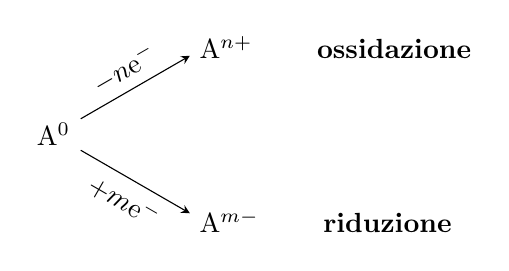
\begin{tikzpicture}
    \node at (0,0) {$\rm A^0$};
    %stato ossidato
    \draw[-stealth,rotate=30] (0.4,0) -- (2,0) node[above=0.1cm,right] {A$^{n+}$ \qquad \textbf{ossidazione}} node[midway, above,rotate=30] {$- n\rm e^-$};
    %stato ridotto
    \draw[-stealth,rotate=-30] (0.4,0) -- (2,0) node[below=0.1cm, right] {A$^{m-}$ \qquad \textbf{riduzione}} node[midway, below,rotate=-30] {$+ m\rm e^-$};
  \end{tikzpicture}
\end{figure}

\comment{
\begin{center}
\schemestart
$\ce{A^0}$\arrow(aa--){->[$\ce{-\;ne^-}$]}[25]$\qquad \qquad \qquad \; \; \ce{A^{n+} \qquad \textbf{ossidazione}}$ 
\arrow(@aa--){->[\hspace{0.1cm}][$\ce{+\;me^-}$]}[-25]$ \qquad \qquad \qquad \ce{A^{m-} \; \; \quad \textbf{riduzione}}$
\schemestop
\end{center}}

\begin{itemize}[leftmargin=0.5cm]
  \item Se ad esso strappiamo un certo numero $n$ di elettroni, esso si caricherà positivamente di una carica $n^+$, in quanto il numero di elettroni non sarà più uguale a quello dei protoni. Allora A si è ossidato ed è diventato catione A$^{n+}$.
  \item Se invece acquista un certo numero $m$ di elettroni, esso si caricherà negativamente di una carica $m^-$. Allora A si è ridotto ed è diventato anione A$^{m-}$.
\end{itemize}

È chiaro che sia catione che anione possono tornare indietro ad A$^0$: il catione può riacquistare gli stessi elettroni ceduti (stavolta si sta riducendo) e l'anione può cedere gli stessi elettroni acquistati (stavolta si sta ossidando):
$$\ce{A^{n+} + ne^- -> A^0} \quad \text{riduzione}$$
$$\ce{A^{m-} - me^- -> A^0} \quad \text{ossidazione}$$
\subsection{Come calcolare il numero di ossidazione?}
Il numero di ossidazione (n.o.) va calcolato per ogni atomo di ogni formula.

\begin{itemize}[leftmargin=0.5cm]
  \item \textbf{Atomi o molecole omonucleari (tipo O$_2$)}
  
  Essi avranno numero di ossidazione pari a zero sempre.
  \begin{center}
    Fe, Zn, $\rm Cl_2$, $\rm O_2$, $\rm N_2$, $\rm P_4$, $\rm S_8$ $\rm n.o.=0$
  \end{center}

  \item \textbf{L'idrogeno (H$_2$ molecola omonucleare)}

  Esso nei suoi composti avrà sempre numero di ossidazione pari a +1, tranne nei composti binari con un metallo (\ce{NaH, CaH_2}) in cui ha stato di ossidazione pari a $-1$.
  \item \textbf{L'ossigeno}

  Esso nei suoi composti avrà sempre numero di ossidazione pari a -2, tranne nei perossidi (composti in cui è presente il gruppo O-O in cui due ossigeni sono legati da un legame covalente, ad esempio l'acqua ossigenata $\rm H_2O_2$) in cui ha numero di ossidazione pari a $-1$.
  \item \textbf{Molecole neutre e ioni}

  Nelle molecole la sommatoria dei numeri di ossidazioni degli atomi che lo compongono deve essere uguale a zero, negli ioni il tale sommatoria è pari alla carica.

  \item \textbf{Fluoro}

  Quando si combina con un altro elemento, il fluoro ha sempre n.o. pari a $-1$.
  \item \textbf{Cloro, bromo e ioduro}

  Hanno n.o. pari a $-1$, tranne quando combinati con ossigeno o fluoro.

  \textbf{ES} $\rm H_2O$

  Mostriamo che $\sum \rm n.o.=0$:

  L'ossigeno ha n.o. pari a $-2$, mentre l'idrogeno ha n.o. pari a $+1$ ma essendocene 2 sarà $2 \times 1$. Sommando si ha
  \begin{center}
    $\sum \rm n.o. = 2\times 1+(-2)=0$
  \end{center}

  \textbf{ES} $\rm H_2O_2$

  Si tratta di un perossido, quindi in questo caso l'ossigeno ha n.o. pari a $-1$. La somma dei numeri di ossidazione è data da
  \begin{center}
    $\sum \rm n.o.=2 \times \text{1+2} \times (-1)=0$
  \end{center}

  \textbf{ES} $\rm ClO_3^-$

  Negli ioni invece la somma dei numeri di ossidazione deve essere uguale alla carica dello ione, per cui si ha
  \begin{center}
  $\sum \rm n.o. = 5+3 \times (-2)=-1$
  \end{center}

\end{itemize}

\newpage
\subsection{Bilanciamento redox}
Per bilanciare una reazione di ossidoriduzione bisogna bilanciare in ordine
\begin{enumerate}
    \item Elettroni scambiati
    \item Cariche
    \item Masse
  \end{enumerate}
\subsubsection{\textbf{ES.1}}
$$\ce{FeCl_3 + SnCl_2 -> FeCl_2 + SnCl_4}$$
$$\text{cloruro ferrico + cloruro stannoso \ce{->} cloruro ferroso + cloruro stannico}$$
Il ferro aveva valenza 2 o 3, ora diremo che ha stato di ossidazione 2 o 3. Lo stagno può essere in forma stannosa o stannica, che corrispondono ad avere stato di ossidazione 2 o 4.

Mettendo insieme questi due reagenti avviene una reazione in cui il cloruro ferrico diventa cloruro ferroso e il cloruro stannoso diventa cloruro stannico. Cos'è accaduto?

Al primo membro c'è $\rm Fe^{3+}$, al secondo $\rm Fe^{2+}$, quindi il ferro ha acquistato un elettrone.

Al primo membro c'è $\rm Sn^{2+}$, al secondo $\rm Sn^{4+}$, quindi lo stagno ha ceduto due elettroni.

\begin{equation*}
  \left.\begin{aligned}
  \ce{Fe^{3+} + e^- -> Fe^{2+}}\\
  \ce{Sn^{2+} -> Sn^{4+} + 2 e^-}
\end{aligned}\right\} \quad \textbf{semireazioni redox}
\end{equation*}

Nella prima semireazione gli elettroni sono a primo membro, nella seconda a secondo membro.

È evidente che se lo stagno cede due elettroni e il ferro ne acquista solo uno, per ogni ione stannoso serviranno due ioni ferrici.
Per bilanciare allora si moltiplicano le specie per gli elettroni scambiati dall'altra.
In questo caso dovremo moltiplicare per 1 i composti dello stagno e per 2 quelli del ferro (in entrambi i membri!):
$$\ce{2 FeCl_3 + SnCl_2 -> 2 FeCl_2 + SnCl_4}$$
Lo stagno ha perso 2 elettroni passando da ione stannoso +2 a ione stannico +4 e si è quindi ossidato. Ossidandosi ha permesso la riduzione del ferro, perché è quello che fornisce gli elettroni. Diciamo quindi che lo stagno è il \textbf{riducente}.

Il ferro ha acquisito un elettrone passando da ione ferrico +3 a ione ferroso +2 e si è quindi ridotto. Riducendosi ha permesso l'ossidazione dello stagno, perché è quello che riceve gli elettroni. Diciamo quindi che il ferro è l'\textbf{ossidante}.

\vspace{0.2cm}Quindi in una reazione redox

\begin{itemize}[leftmargin=0.5cm]
  \item la specie che si ossida è il riducente;
  \item la specie che si riduce è l'ossidante.
\end{itemize}

Ricorda: a meno che non si agisca con metodi elettro-chimici, nelle reazioni redox è indispensabile che ci siano sia ossidante che riducente. Non può esserci solo una tra le due specie, altrimenti la reazione non avverrà. Questo equivale a dire che le specie chimiche non devono trovarsi tutte al più alto o al più basso stato di ossidazione.

Vediamo perché con degli esempi:

\begin{itemize}[leftmargin=0.5cm]
  \item Se mettiamo a reagire cloruro ferrico $\rm FeCl_3$ e cloruro stannico $\rm SnCl_4$ non si avrà nessun tipo di reazione, né di scambio perché in entrambi i composti l'anione è il cloruro, né redox perché il ferro è nel suo più alto stato di ossidazione in cui può solo ricevere elettroni e altrettanto vale per lo stagno, quindi non c'è nessuno che cede elettroni:
  $$\ce{FeCl_3 + SnCl_4 ->}\text{nessuna reazione}$$
  \item Se invece mettiamo a reagire cloruro ferroso $\rm FeCl_2$ e cloruro stannoso $\rm SnCl_2$ anche in questo caso non si avrà alcuna reazione, perché il ferro è nel suo più basso stato di ossidazione in cui può solo cedere elettroni e altrettanto vale per lo stagno, quindi non c'è nessuno che acquista elettroni.
$$\ce{FeCl_2 + SnCl_2 ->}\text{nessuna reazione}$$
\end{itemize}
\subsubsection{\textbf{ES.2}}
$$\ce{KMnO_4 + FeSO_4 + H_2SO_4 -> MnSO_4 + Fe_2(SO_4)_3 + K_2SO_4 + H_2O}$$
$$\text{permanganato di potassio + solfato ferroso + acido solforico \ce{->}}$$
$$\ce{->}\text{solfato di manganese (II) + solfato ferrico + solfato di potassio + acqua}$$
Sono tutte specie solubili in acqua, pertanto in acqua sono dissociate. In particolare li troveremo come

$$\ce{KMnO_4 -> K^+ + MnO_4^-}$$
$$\ce{FeSO_4 -> Fe^{2+} + SO_4^{2-}}$$
$$\ce{H_2SO_4 -> 2 H^+ + SO_4^{2-}}$$
$$\ce{MnSO_4 -> Mn^{2+} + SO_4^{2-}}$$
$$\ce{Fe_2(SO_4)_3 -> 2 Fe^{3+} + 3 SO_4^{2-}}$$
$$\ce{K_2SO_4 -> 2 K^+ + SO_4^{2-}}$$
A questo punto inizio a guardare i numeri di ossidazione di tutti gli elementi di ogni composto per capire quali partecipano alla reazione, in modo da lavorare al bilanciamento su una reazione semplificata per poi tornare a quella completa.

Lo ione $\rm K^+$ resta tale anche al secondo membro, quindi non partecipa all'ossidoriduzione. Analogamente, lo zolfo resta ione solfato $\rm SO_4^{2-}$ nei composti del secondo membro. Pertanto non li scriveremo nella reazione semplificata, dove invece metteremo tutti gli altri ioni e in più sia l'idrogeno $\rm H^+$ che l'acqua, i quali servono per il bilancio delle cariche e della massa:
$$\ce{MnO_4- + 2Fe^2+ + H+ -> Mn^2+ + 2Fe^3+ + H_2O}$$
Iniziamo a ragionare sui numeri di ossidazione.

Al primo membro il manganese si trova nello ione permanganato $\rm MnO_4^-$. L'ossigeno ha stato di ossidazione $-2$, per 4 atomi in totale -8. Affinché lo ione abbia carica totale -1 il manganese deve avere stato di ossidazione $+7$ ($4\times(-2) + 7 = -1$). Al secondo membro invece ha n.o. pari a +2, ciò significa che ha acquistato 5 elettroni e quindi si è ridotto:
$$\ce{Mn^7+ -> Mn^2+ \; \text{(+5e)}}$$
Per il ferro dobbiamo innanzitutto notare che al secondo membro ci sono 2 atomi, per cui dobbiamo moltiplicare per 2 il ferro al primo membro (ecco perché nella reazione semplificata c'è $\rm 2Fe^{2+}$). Al primo membro è ione ferroso $\rm Fe^{2+}$, al secondo ione ferrico $\rm Fe^{3+}$, ciò significa che ha ceduto 1 elettrone e quindi si sta ossidando
$$\ce{2Fe^2+ -> 2Fe^3+ \; \text{(-2e)}}$$
A questo punto moltiplichiamo gli ioni di una specie per il numero di elettroni scambiati dall'altra specie. In questo caso moltiplichiamo per 5 gli ioni del ferro e per 2 quelli del manganese:
$$\ce{2MnO_4- + 10Fe^2+ + H+ -> 2Mn^2+ + 10Fe^3+ + H_2O}$$
Arrivati a questo punto gli elettroni sono bilanciati. Il prossimo passo è quello di bilanciare le cariche.

Per fare ciò contiamo le cariche del secondo membro: i 2 ioni $\rm Mn^{2+}$ danno 4 cariche positive, i 10 ioni $\rm Fe^{3+}$ 30 cariche positive. Entrambi sono termini positivi che si sommano, per un totale di 34 cariche positive. Siccome ci deve essere l'equilibrio, dobbiamo averne un numero uguale anche al primo membro. In questo ci sono 2 ioni $\rm MnO_4^-$ che danno due cariche negative e 10 ioni $\rm Fe^{2+}$ che danno 20 cariche positive. In questo caso si sottraggono per un totale di 18 cariche positive. La differenza è di 16 cariche. L'unica cosa che posso usare per aggiustare le cariche è lo ione $\rm H^+$, quindi moltiplichiamo questo per la differenza, cioè per 16:
$$\ce{2MnO_4- + 10Fe^2+ + 16H+ -> 2Mn^2+ + 10Fe^3+ + H_2O}$$
Le cariche saranno così bilanciate.

A questo punto mettiamo questi numeri nella reazione completa, in modo da bilanciare le masse:
$$\ce{2KMnO_4 + 10FeSO_4 + 8H_2SO_4 -> 2MnSO_4 + 5Fe_2(SO_4)_3 + K_2SO_4 + 8H_2O}$$
Attenzione: alcuni numeri vengono dimezzati, a causa della specie molecolare. Ad esempio, il solfato ferrico ha $\rm Fe_2$ quindi moltiplico per 5 anziché per 10. Infine le 8 molecole di acqua derivano dal fatto che al primo membro abbiamo 16 ioni $\rm H^+$ e 8 ossigeni provenienti dal permanganato.

\vspace{0.2cm}\subsubsection{\textbf{ES.3}}
$$\ce{K_2Cr_2O_7 + KI + H_2SO_4 -> Cr_2(SO_4)_3 + I_2 + K_2SO_4 + H_2O}$$
$$\text{bicromato di potassio + ioduro di potassio + acido solforico \ce{->}}$$
$${\ce{->} \text{solfato di cromo (III) +  iodio + solfato di potassio + acqua}}$$
Le dissociazioni di questi composti sono
$$\ce{K_2Cr_2O_7 -> 2K^+ + Cr_2O_7^2-}$$ 
$$\ce{KI -> K+ + I-}$$
$$\ce{H_2SO_4 -> 2H+ + SO_4^2-}$$
$$\ce{Cr_2(SO_4)_3 -> 2Cr^3+ + 3SO_4^2-}$$
$$\ce{I_2 -> 2I^{(0)}}$$
$$\ce{K_2SO_4 -> 2K+ + SO_4^2-}$$
Il cromo nello ione bicromato mostra n.o. +6, mentre a secondo membro +3. Ha quindi acquistato 3 elettroni, riducendosi.
Lo iodio mostra n.o. pari a $-1$ nel primo membro perché si trova in un idruro, pari a 0 nel secondo perché è in forma molecolare. Ha quindi perso un elettrone, ossidandosi.

Gli ioni $\rm K^+$ e $\rm SO_4^2-$ invece hanno stesso n.o. sia a primo che a secondo membro.

Per il cromo non abbiamo problemi col numero di atomi, per lo iodio si perché a destra è in forma molecolare $\rm I_2$, per cui devo moltiplicare per 2 lo ione $\rm I^+$.

La reazione semplificata allora sarà
$$\ce{Cr_2O_7^2- + 2I^- + H+ -> 2Cr^3+ + I_2 + H_2O}$$
Ragioniamo ora sullo scambio di elettroni:
$$\ce{2Cr^6+ -> 2Cr^3+ \; \text{(+6e, 3 per ciascuno ione)}}$$
$$\ce{2I- -> I_2 \; \text{(-2e, 1 per ciascuno ione)}}$$
In questo caso 6 e 2 possono essere semplificati, diventando 3 e 1.

Moltiplichiamo quindi le specie dello iodio per 3 e quelle del cromo per 1:
$$\ce{Cr_2O_7^2- + 6I^- + H+ -> 2Cr^3+ 3I_2 + H_2O}$$
A questo punto gli elettroni sono bilanciati.

Bilanciamo le cariche.

Al secondo membro abbiamo due ioni $\rm Cr^{3+}$, quindi abbiamo 2$\times$3=6 cariche positive, che voglio anche al primo membro. In questo ci sono 2 cariche negative dello ione bicromato e altre 6 cariche negative degli ioduri, per un totale di 8 cariche negative. Per bilanciare allora ci servono 14 ioni $\rm H^+$. Inoltre possiamo anche bilanciare le masse, perché 14 ioni $\rm H^+$ e 7 ioni $\rm O^{2-}$ danno 7 molecole di acqua:
$$\ce{Cr_2O_7^2- + 6I^- + 14H+ -> 2Cr^3+ 3I_2 + 7H_2O}$$
Riportiamo questi numeri nella reazione completa:
$$\ce{K_2Cr_2O_7 + 6KI + 7H_2SO_4 -> Cr_2(SO_4)_3 + 3I_2 + 4K_2SO_4 + 7H_2O}$$
Attenzione! La molecola $\rm K_2SO_4$ non ha partecipato alla redox, quindi per ottenere il suo coefficiente stechiometrico abbiamo dovuto contare quanto potassio e quanti ioni solfati ci sono al primo membro.

\vspace{0.2cm}Le reazioni viste finora avvengono in ambiente acido, ossia per bilanciare dobbiamo aggiungere ioni $\rm H^+$. Se avvenissero in ambiente basico, per bilanciare servirebbero ioni $\rm OH^-$.
\subsubsection{\textbf{ES.4: reazioni con due ossidanti}}
$$\ce{KMnO_4 + H_2O_2 + H_2SO_4 -> MnSO_4 + O_2 + K_2SO_4 + H_2O}$$
$$\text{permanganato di potassio + perossido di idrogeno + acido solforico }\ce{->}$$
$$\ce{->}\text{solfato di manganese (II) + solfato di potassio + acqua}$$
Se mettiamo insieme due ossidanti (che possono dar luogo a una reazione a patto che non siano entrambi nel loro più alto stato di ossidazione) essi si trovano in competizione: quello più forte sarà l'ossidante, l'altro si comporterà come un riducente. In questo esempio gli ossidanti sono il permanganato e l'acqua ossigenata ($\rm H_2O_2$), il più forte è il primo.

Le dissociazioni delle molecole sono
$$\ce{KMnO_4 -> K+ + MnO_4-}$$
$$\ce{H_2O_2 -> 2H+ + 2O-}$$
$$\ce{H_2SO_4 -> 2H+ + SO_4^2-}$$
$$\ce{MnSO_4 -> Mn^2+ + SO_4^2-}$$
$$\ce{O_2 -> 2O^{(0)} \text{(non si dissocia in acqua!)}}$$
$$\ce{K_2SO_4 -> 2K+ + SO_4^2-}$$
Il manganese passa da n.o. +7 nel permanganato a n.o. +2 nel solfato, dunque ha acquistato 5 elettroni e si è ridotto. L'ossigeno passa da -1 nel perossido a 0 in forma molecolare, dunque ha perso un elettrone e si è ossidato. Tutte le altre specie mantengono inalterato il loro n.o. e quindi non partecipano alla redox.

La reazione semplificata allora sarà
$$\ce{MnO_4- + H_2O_2 + H+ -> Mn^2+ + O_2 + H_2O}$$

Ragioniamo sugli elettroni scambiati
$$\begin{cases}
    \ce{Mn^{+7} +5e -> Mn^{+2}}\\
    \ce{2O^{-1} -> 2O^{(0)} +2e} \quad \text{(1 per ciascuno ione)}
\end{cases}$$
Moltiplichiamo quindi per 5 le specie dell'ossigeno e per 2 quelle del manganese:
$$\ce{2MnO_4- + 5H_2O_2 + H+ -> 2Mn^2+ + 5O_2 + H_2O}$$
Bilanciamo le cariche.

A secondo membro 2 ioni $\rm Mn^{2+}$ danno 4 cariche positive, ma al primo membro ci sono solo 2 cariche negative dato dai due ioni $\rm MnO_4^-$. Servono quindi 2 cariche positive per neutralizzarle e altre 4 per bilanciare, quindi aggiungiamo in totale 6 ioni $\rm H^+$. Possiamo bilanciare anche le masse, la reazione sarà:
$$\ce{2MnO_4- + 5H_2O_2 + 6H+ -> 2Mn^2+ + 5O_2 + 8H_2O}$$
Attenzione! abbiamo ottenuto 8 molecole di acqua perché i 5 perossidi danno 10 atomi di idrogeno e quindi in totale ne abbiamo 16.

Riportando i numeri nella reazione completa otteniamo il bilanciamento:
$$\ce{2KMnO_4 + 5H_2O_2 + 3H_2SO_4 -> 2MnSO_4 + 5O_2 + K_2SO_4 + 8H_2O}$$
(Il coefficiente stechiometrico dell'acido solforico è 3 e non 6 perché ogni molecola contiene 2 idrogeni)
\subsubsection{\textbf{ES.5: reazioni di disproporzione (o dismutazione)}}

Sono reazioni in cui una stessa specie chimica in parte si ossida e in parte si riduce.
$$\ce{Cl_2 + NaOH -> NaCl + NaClO + H_2O}$$
$$\text{cloro + idrossido di sodio \ce{->} cloruro di sodio + ipoclorito di sodio + acqua}$$
Questa è una reazione che avviene a freddo in ambiente basico, per cui stavolta al posto dell'$\rm H^+$ ci sarà l'$\rm OH^-$.

Le dissociazioni che avvengono sono:
$$\ce{Cl_2 -> 2Cl^{(0)}}$$
$$\ce{NaOH -> Na+ + OH-}$$
$$\ce{NaCl -> Na+ + Cl-}$$
$$\ce{NaClO -> Na+ + ClO-}$$
In questa reazione il cloro a primo membro ha n.o. 0 perché si trova in forma molecolare, a secondo membro ha n.o. +1 nell'ipoclorito (affinché lo ione $\rm ClO^-$ abbia n.o. -1 dato che l'ossigeno ha n.o. pari a -2 il cloro deve averlo proprio uguale a +1) e -1 nel cloruro. Ciò che avviene è che un atomo di cloro cede un elettrone all'altro, per cui il primo diventa $\rm Cl^+$ e si ossida, il secondo diventa $\rm Cl^-$ e si riduce.
$$\ce{Cl^0 -> Cl+} \; \text{(-1e)}$$
$$\ce{Cl^0 ->Cl-} \; \text{(+1e)}$$
Il sodio invece resta \ce{Na+} e quindi non partecipa alla redox.

La reazione semplificata è
$$\ce{Cl_2 + OH- -> Cl- + ClO- + H_2O}$$
È chiaro che gli elettroni sono già bilanciati. Bilanciamo le cariche.

Al secondo membro abbiamo 2 cariche negative mentre al primo nessuna, dunque servono due gruppi \ce{OH-} al primo membro:
$$\ce{Cl_2 + 2OH- -> Cl- + ClO- + H_2O}$$
Riportiamo i numeri nella reazione completa
$$\ce{Cl_2 + 2NaOH -> NaCl + NaClO + H_2O}$$
Immaginiamo ora che l'acqua in cui avviene la reazione non sia fredda: la reazione va avanti. Il cloro da una parte acquista elettroni diventando cloruro, dall'altra perde elettroni diventando clorato:
$$\ce{Cl_2 + NaOH -> NaCl + NaClO_3 + H_2O}$$
Nel clorato il cloro ha n.o. pari a +5 (affinché la molecola \ce{NaClO_3} sia neutra, dato che Na ha n.o. pari a +1 e 3 ossigeni danno un n.o. pari a -6, il cloro deve avere n.o. +5), cioè perde più elettroni rispetto al caso precedente (in altre parole questa ossidazione è più spinta).

La reazione semplificata sarà
$$\ce{Cl_2 + OH- -> Cl- + ClO_3- + H_2O}$$
Ragioniamo sugli elettroni scambiati.
$$\ce{Cl^{(0)} ->Cl-} \; \text{(+1e)}$$
$$\ce{Cl^{(0)} ->Cl^5+} \; \text{(-5e)}$$
Dobbiamo quindi moltiplicare per 5 la specie cloruro e per 1 la specie clorato. Per ottenere il numero di atomi di cloro a primo membro basta fare la somma degli atomi totali di cloro a destra: $5+1=6$
$$\ce{3Cl_2 + OH- -> 5Cl- + ClO_3- + H_2O}$$
(Il cloro è moltiplicato per 3 perché ogni molecola contiene 2 atomi)

Bilanciamo le cariche. A secondo membro abbiamo 5 cariche negative del cloruro e 1 carica negativa del clorato, per un totale di 6 cariche negative. A primo non ci sono cariche, quindi per bilanciare aggiungiamo 6 ioni $\rm OH^-$. Avendo usato 3 ossigeni nel clorato, ne restano altri 3 con cui formiamo 3 molecole di acqua
$$\ce{3Cl_2 + 6OH- -> 5Cl- + ClO_3- + 3H_2O}$$
Portiamo i numeri nella reazione completa:
$$\ce{3Cl_2 + 6NaOH -> 5NaCl + NaClO_3 + 3H_2O}$$